
                \documentclass[8pt]{beamer}
                \usepackage{beamerthemesplit}
                %\usepackage[orientation=portrait,size=custom,width=60,height=80, scale = 1.4]{beamerposter} 
                \geometry{papersize={16cm,22cm}}
                \usetheme{CambridgeUS} 
                \usepackage{textpos} 
                \usepackage[latin1]{inputenc} 
                \usepackage{amsmath} 
                \usepackage{mathtools} 
                \usepackage{color} 
                \usepackage{mathabx} 
                \usepackage{microtype} % Miglioramento dell'allineamento del testo
                \usepackage{ragged2e} % Miglioramento dell'allineamento del testo
                \usepackage{graphicx}
                \usepackage{longtable} 
                \usepackage{tikz} 
                \usepackage{esvect} 
                \usetikzlibrary{arrows,shapes} 
                \usecolortheme{beaver} 
                \usepackage{graphicx} 
                \usepackage{booktabs}
                \usepackage{changepage} 
                \setbeamertemplate{navigation symbols}{} 
                \setbeamertemplate{navigation symbols}{} 
            
        \title{GEANT4 Simulation Report}
        \author{Riccardo Nicolaidis \footnote{riccardo.nicolaidis@unitn.it}}
        \date{\today}
        
        \begin{document}
        
            \begin{frame}
                \titlepage
            \end{frame}
            
            \begin{frame}
                \frametitle{Info}
            
                \centering
                GDML File Name : \textbf{ LEM\_Plastic\_Mirion\_Ametek-worldVOL\_Parsed.gdml}
                
                
                \vspace{2 cm}
                \textbf{NTuple Info}:
                \vspace{1 cm}
                
        \begin{itemize}
        
        \item Ntuple ID: 0 Ntuple Name: Edep
        
        \item Ntuple ID: 0 Ntuple Column ID: 0 Ntuple Column Name: RandEnergy
        
        \item Ntuple ID: 0 Ntuple Column ID: 1 Ntuple Column Name: Xgen
        
        \item Ntuple ID: 0 Ntuple Column ID: 2 Ntuple Column Name: Ygen
        
        \item Ntuple ID: 0 Ntuple Column ID: 3 Ntuple Column Name: Zgen
        
        \item Ntuple ID: 0 Ntuple Column ID: 4 Ntuple Column Name: pDirX
        
        \item Ntuple ID: 0 Ntuple Column ID: 5 Ntuple Column Name: pDirY
        
        \item Ntuple ID: 0 Ntuple Column ID: 6 Ntuple Column Name: pDirZ
        
        \item Ntuple ID: 0 Ntuple Column ID: 7 Ntuple Column Name: Ed\_LV\_Calo
        
        \item Ntuple ID: 0 Ntuple Column ID: 8 Ntuple Column Name: Ed\_LV\_PlasticVetoTop
        
        \item Ntuple ID: 0 Ntuple Column ID: 9 Ntuple Column Name: Ed\_LV\_SiliconDetector\_Thin\_4
        
        \item Ntuple ID: 0 Ntuple Column ID: 10 Ntuple Column Name: Ed\_LV\_SiliconDetector\_Thin\_1
        
        \item Ntuple ID: 0 Ntuple Column ID: 11 Ntuple Column Name: Ed\_LV\_SiliconDetector\_Thin\_2
        
        \item Ntuple ID: 0 Ntuple Column ID: 12 Ntuple Column Name: Ed\_LV\_SiliconDetector\_Thin\_0
        
        \item Ntuple ID: 0 Ntuple Column ID: 13 Ntuple Column Name: Ed\_LV\_SiliconDetector\_Thin\_3
        
        \item Ntuple ID: 0 Ntuple Column ID: 14 Ntuple Column Name: Ed\_LV\_SiliconDetector\_Thick\_3
        
        \item Ntuple ID: 0 Ntuple Column ID: 15 Ntuple Column Name: Ed\_LV\_SiliconDetector\_Thick\_1
        
        \item Ntuple ID: 0 Ntuple Column ID: 16 Ntuple Column Name: Ed\_LV\_SiliconDetector\_Thick\_2
        
        \item Ntuple ID: 0 Ntuple Column ID: 17 Ntuple Column Name: Ed\_LV\_PlasticVetoBottom
        
        \item Ntuple ID: 0 Ntuple Column ID: 18 Ntuple Column Name: Ed\_LV\_SiliconDetector\_Thick\_4
        
        \item Ntuple ID: 0 Ntuple Column ID: 19 Ntuple Column Name: Ed\_LV\_SiliconDetector\_Thick\_0
        
        \end{itemize}
        
            \end{frame}
            
            \begin{frame}
                \frametitle{Material Info}
            
            \begin{table}
            \begin{tabular}{lll}
             Volume & Material & Mass (g) \\
                    
            \midrule
            LV\_AlTop & G4\_Al & 532.446\\
                        LV\_BakeliteCable\_1 & G4\_BAKELITE & 0.327105\\
                        LV\_BakeliteCable\_3 & G4\_BAKELITE & 0.327105\\
                        LV\_AlFrame\_Thick\_3 & G4\_Al & 2.97844\\
                        LV\_BakeliteCable & G4\_BAKELITE & 0.242643\\
                        LV\_BakeliteCable\_4 & G4\_BAKELITE & 0.327105\\
                        LV\_AlFrame\_Thick\_1 & G4\_Al & 2.97844\\
                        LV\_AlFrame\_Thick\_2 & G4\_Al & 2.97844\\
                        LV\_AlScrew\_Thick\_2 & G4\_Al & 2.44318\\
                        LV\_AlScrew\_Thick\_3 & G4\_Al & 2.44318\\
                        LV\_BakeliteBoardMiddleUpper & G4\_BAKELITE & 18.9792\\
                        LV\_BakeliteBoardCalo & G4\_BAKELITE & 7.99125\\
                        LV\_AlCoverLower & G4\_Al & 22.6611\\
                        LV\_Calo & G4\_PLASTIC\_SC\_VINYLTOLUENE & 74.304\\
                        LV\_PlasticVetoTop & G4\_PLASTIC\_SC\_VINYLTOLUENE & 235.225\\
                        LV\_BakeliteBoardBottom & G4\_BAKELITE & 19.1034\\
                        LV\_AlFrame\_Thin\_2 & G4\_Al & 2.29301\\
                        LV\_SiliconDetector\_Thin\_4 & G4\_Si & 0.0325397\\
                        LV\_AlFrame\_Thin\_3 & G4\_Al & 2.29301\\
                        LV\_AlFrame\_Thin\_4 & G4\_Al & 2.29301\\
                        LV\_AlCoverUpper & G4\_Al & 21.9613\\
                        LV\_SiliconDetector\_Thin\_1 & G4\_Si & 0.0325397\\
                        LV\_SiliconDetector\_Thin\_2 & G4\_Si & 0.0325397\\
                        LV\_AlFrame\_Thin\_0 & G4\_Al & 1.30068\\
                        LV\_SiliconDetector\_Thin\_0 & G4\_Si & 0.0104495\\
                        LV\_AlFrame\_Thin\_1 & G4\_Al & 2.29301\\
                        LV\_SiliconDetector\_Thin\_3 & G4\_Si & 0.0325397\\
                        LV\_BakeliteCable\_2 & G4\_BAKELITE & 0.327105\\
                        LV\_SiliconDetector\_Thick\_3 & G4\_Si & 0.135903\\
                        LV\_SiliconDetector\_Thick\_1 & G4\_Si & 0.135903\\
                        LV\_SiliconDetector\_Thick\_2 & G4\_Si & 0.135903\\
                        LV\_AlBottom & G4\_Al & 422.153\\
                        LV\_BakeliteBoardMiddleLower & G4\_BAKELITE & 15.0798\\
                        LV\_PlasticVetoBottom & G4\_PLASTIC\_SC\_VINYLTOLUENE & 128.504\\
                        LV\_AlScrew\_1 & G4\_Al & 5.5011\\
                        LV\_AlScrew & G4\_Al & 5.5011\\
                        LV\_AlScrew\_2 & G4\_Al & 5.5011\\
                        LV\_AlScrew\_3 & G4\_Al & 5.5011\\
                        LV\_AlScrew\_Thick\_1 & G4\_Al & 2.44318\\
                        LV\_AlFrame\_Thick\_4 & G4\_Al & 2.97844\\
                        LV\_AlScrew\_Thick\_0 & G4\_Al & 1.46527\\
                        LV\_SiliconDetector\_Thick\_4 & G4\_Si & 0.135903\\
                        LV\_AlFrame\_Thick\_0 & G4\_Al & 2.18948\\
                        LV\_SiliconDetector\_Thick\_0 & G4\_Si & 0.0439621\\
                        LV\_AlScrew\_Thick\_4 & G4\_Al & 2.44318\\
                        
            \bottomrule
            \end{tabular}
            \end{table}
            
            \end{frame}
            
            \begin{frame}
                \frametitle{PID}
            
        \begin{figure}[h]
            \centering
            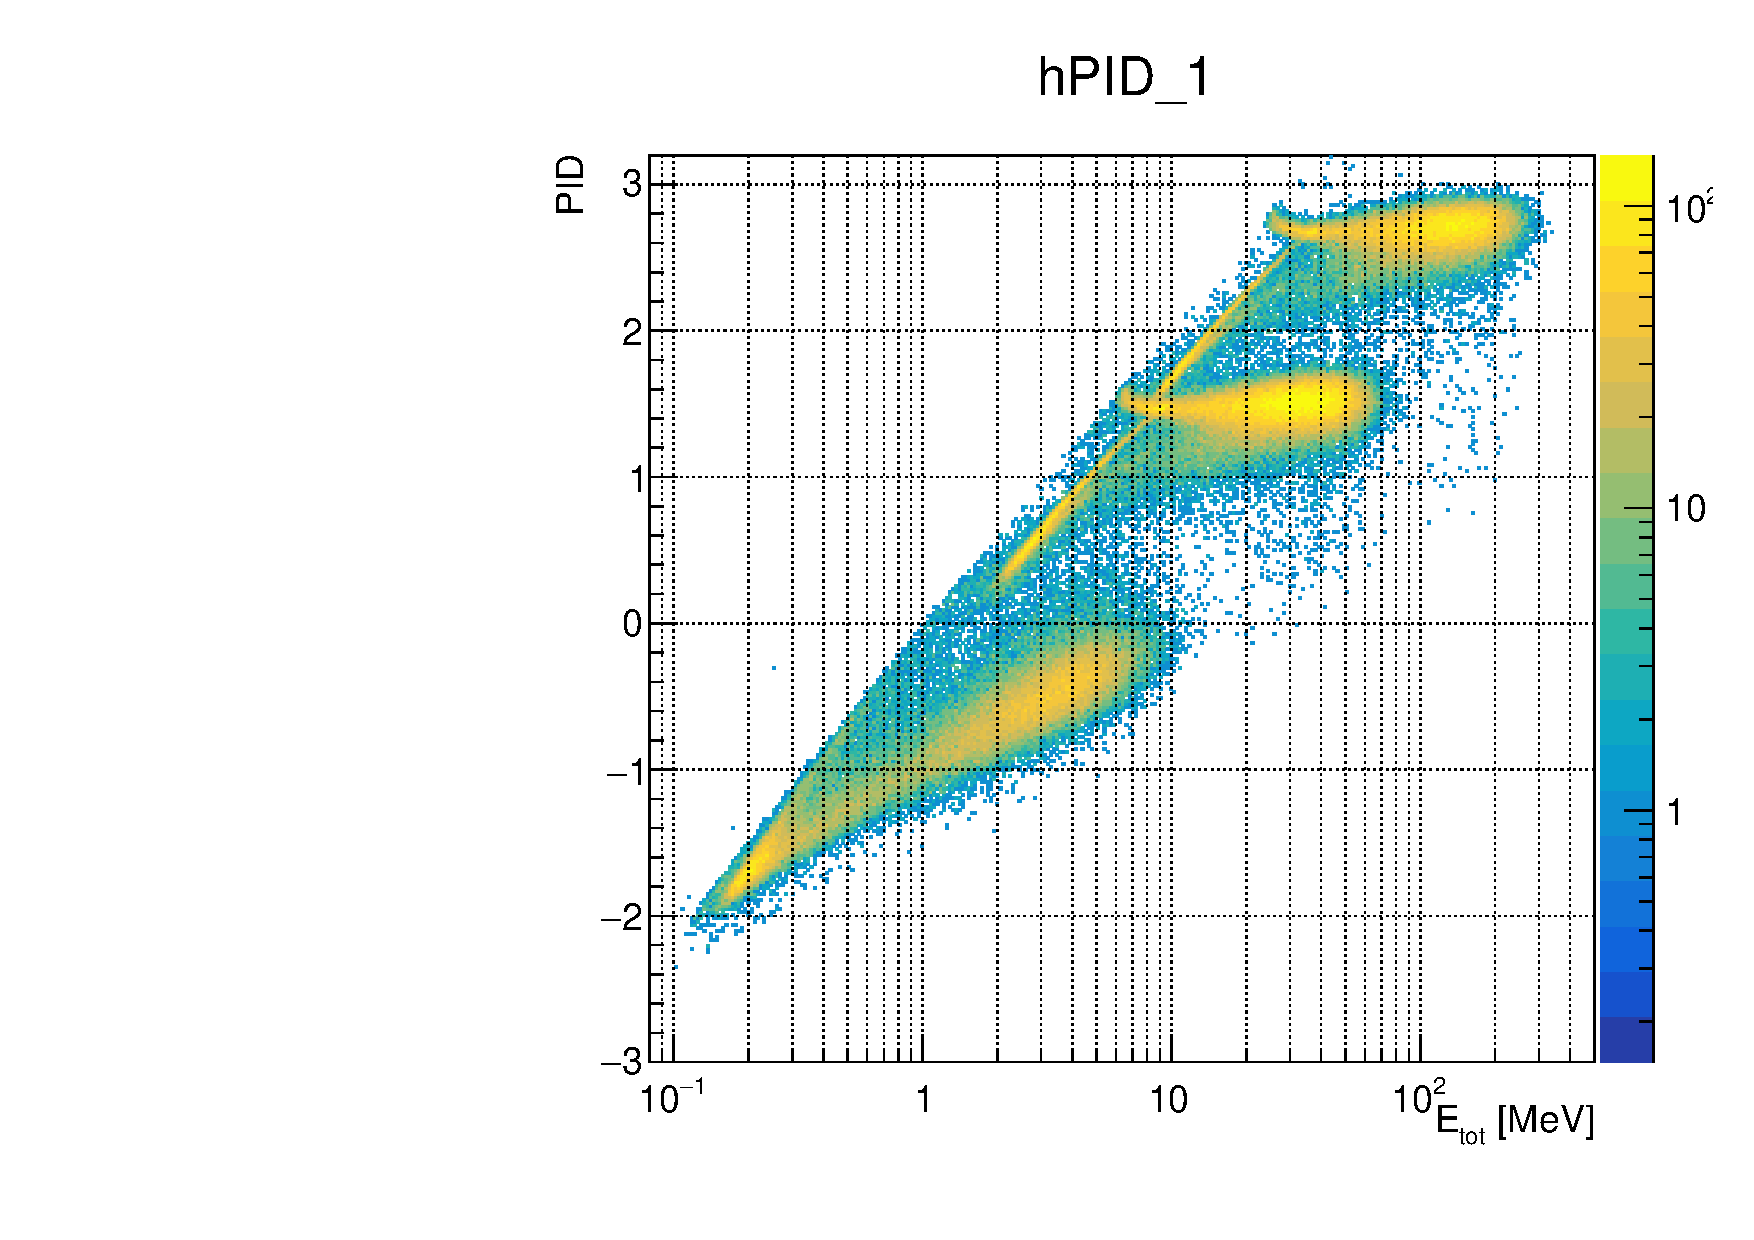
\includegraphics[width=1.0\textwidth]{/home/riccardo/Documenti/GeantProjects/LEM\_GDML\_upgrade/Output\_Geant4Simulation\_20230814/Analysis\_output/GDML\_file\_4/PID\_plots/gPID.pdf}
            \caption{PID, No Gaussian Smearing, Total Energy is the Energy reconstructed.}
        \end{figure}
        
            \end{frame}
            
            \begin{frame}
                \frametitle{PID No Calorimeter}
            
        \begin{figure}[h]
            \centering
            \includegraphics[width=1.0\textwidth]{/home/riccardo/Documenti/GeantProjects/LEM\_GDML\_upgrade/Output\_Geant4Simulation\_20230814/Analysis\_output/GDML\_file\_4/PID\_plots/PID\_NoCalo.pdf}
            \caption{PID, No Gaussian Smearing, Total Energy is the Energy reconstructed, No Calorimeter.}
        \end{figure}
        
            \end{frame}
            
            \begin{frame}
                \frametitle{PID MC Energy}
            
        \begin{figure}[h]
            \centering
            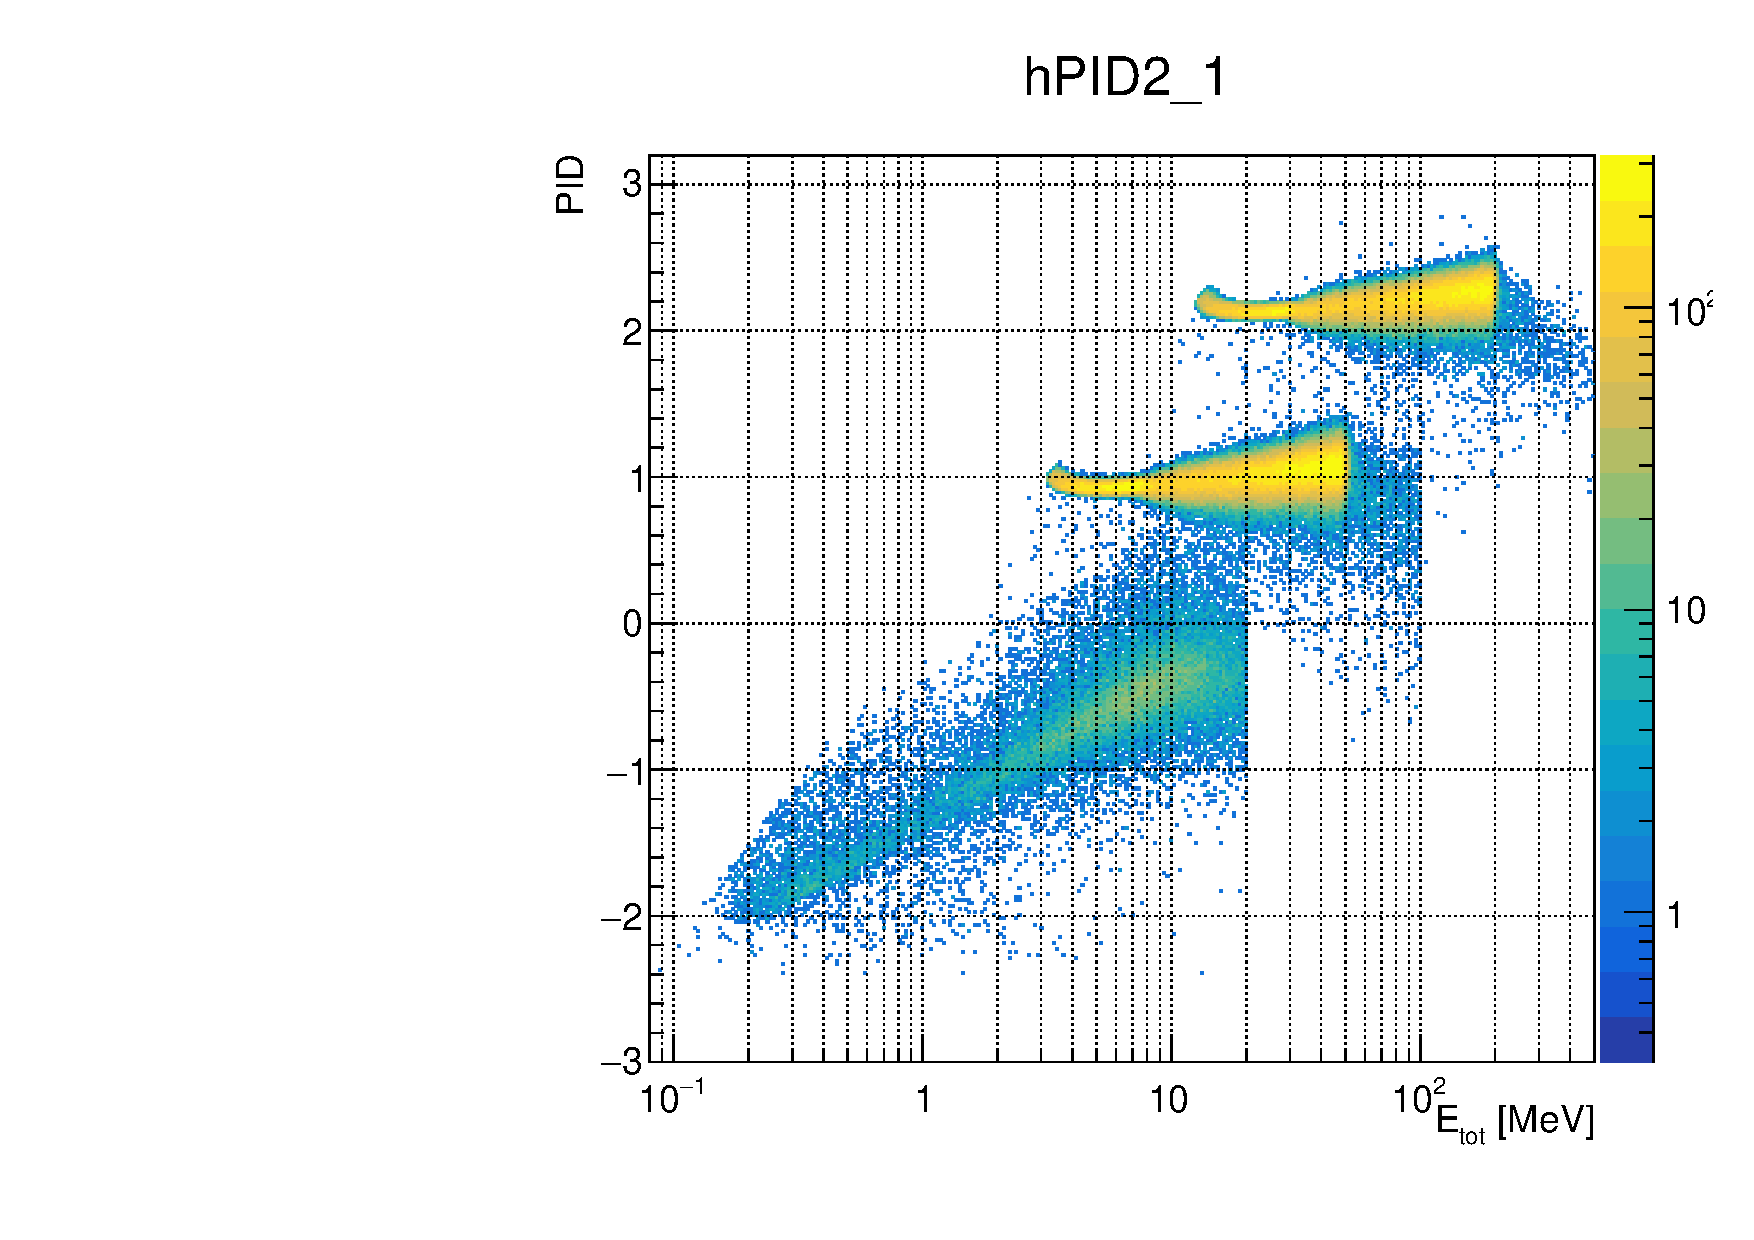
\includegraphics[width=1.0\textwidth]{/home/riccardo/Documenti/GeantProjects/LEM\_GDML\_upgrade/Output\_Geant4Simulation\_20230814/Analysis\_output/GDML\_file\_4/PID\_plots/gPID2.pdf}
            \caption{PID, No Gaussian Smearing, Total Energy is the MC Energy.}
        \end{figure}
        
            \end{frame}
            
            \begin{frame}
                \frametitle{PID MC Energy No Calorimeter}
            
        \begin{figure}[h]
            \centering
            \includegraphics[width=1.0\textwidth]{/home/riccardo/Documenti/GeantProjects/LEM\_GDML\_upgrade/Output\_Geant4Simulation\_20230814/Analysis\_output/GDML\_file\_4/PID\_plots/PID2\_NoCalo.pdf}
            \caption{PID, No Gaussian Smearing, Total Energy is the MC Energy, No Calorimeter.}
        \end{figure}
        
            \end{frame}
            
            \begin{frame}
                \frametitle{PID Gaussian Smearing}
            
        \begin{figure}[h]
            \centering
            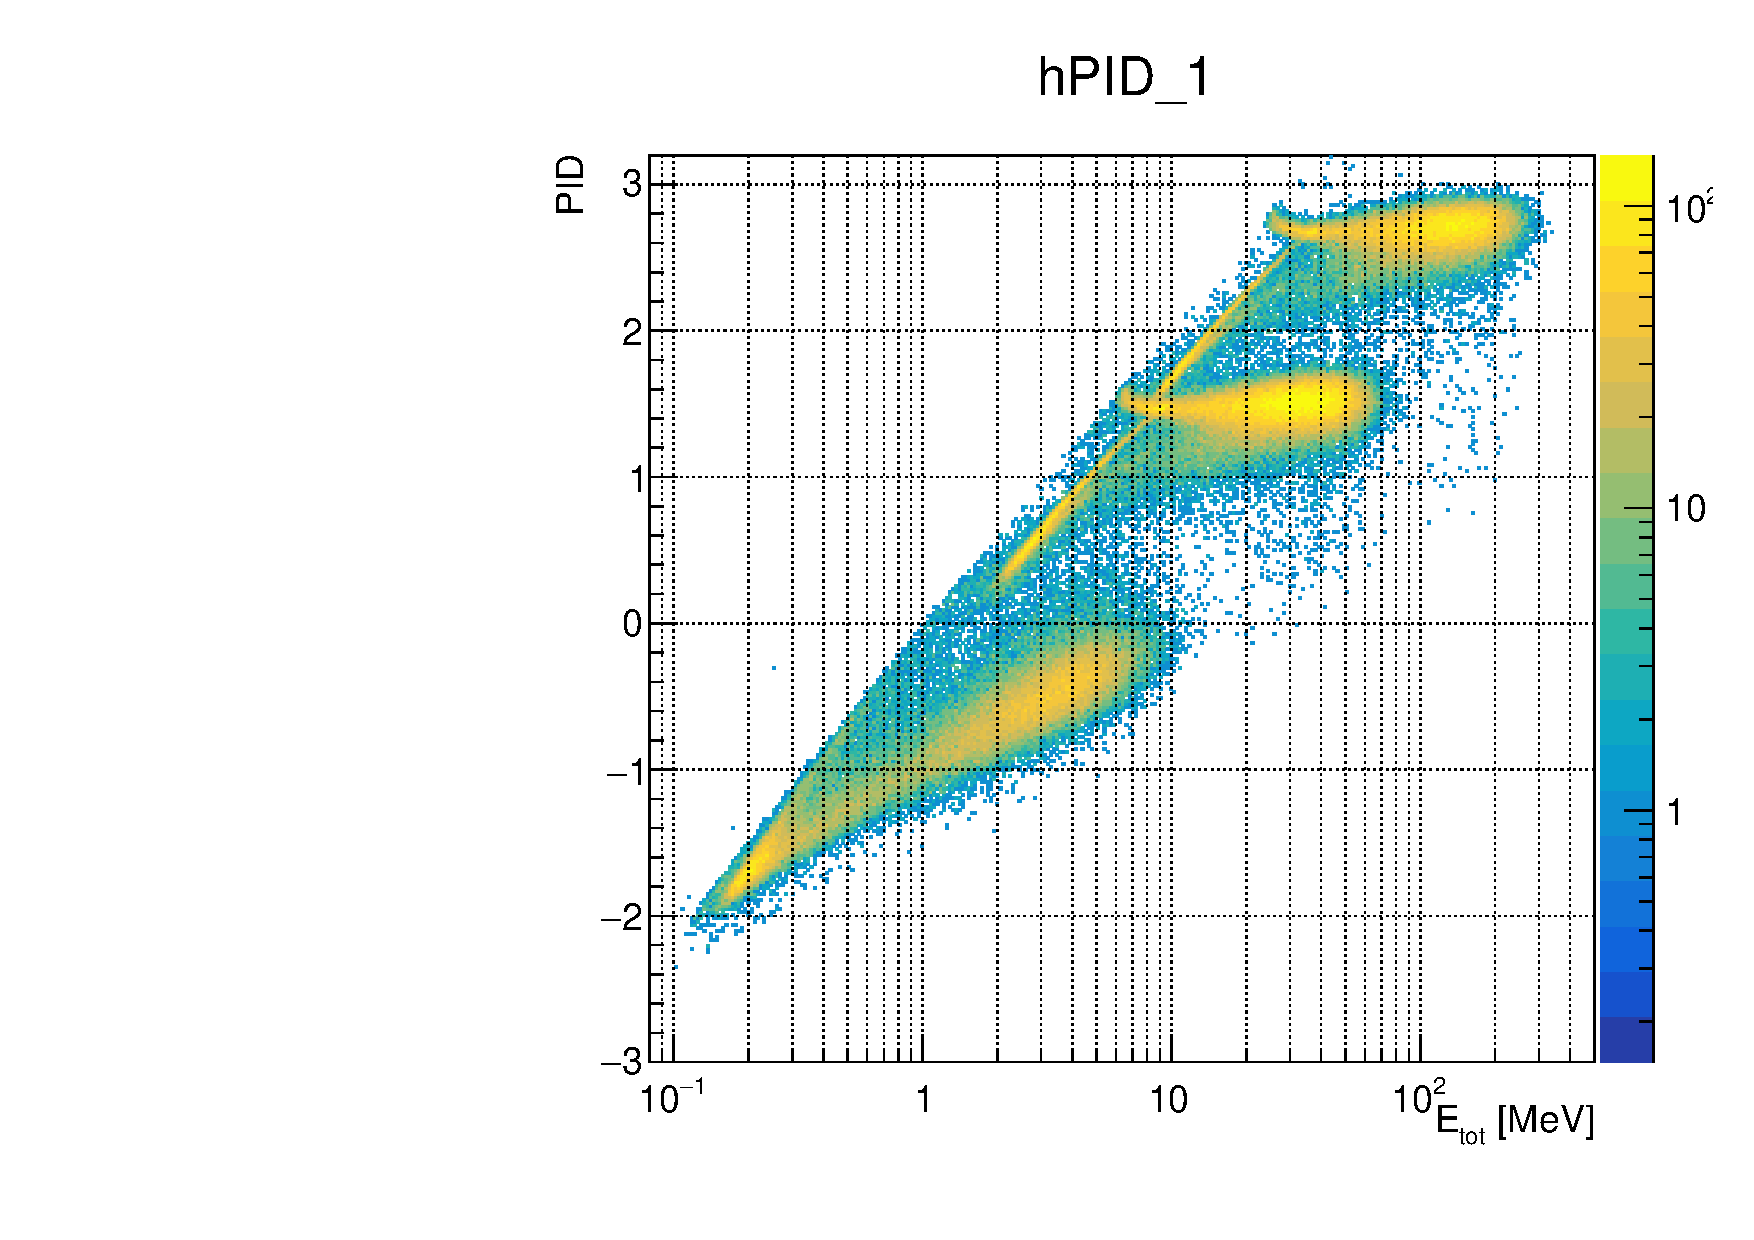
\includegraphics[width=1.0\textwidth]{/home/riccardo/Documenti/GeantProjects/LEM\_GDML\_upgrade/Output\_Geant4Simulation\_20230814/Analysis\_output/GDML\_file\_4/PID\_plots/gPID.pdf}
            \caption{PID, Gaussian Smearing, Total Energy is the Energy reconstructed.}
        \end{figure}
        
            \end{frame}
            
            \begin{frame}
                \frametitle{PID Gaussian Smearing No Calorimeter}
            
        \begin{figure}[h]
            \centering
            \includegraphics[width=1.0\textwidth]{/home/riccardo/Documenti/GeantProjects/LEM\_GDML\_upgrade/Output\_Geant4Simulation\_20230814/Analysis\_output/GDML\_file\_4/PID\_plots/gPID\_NoCalo.pdf}
            \caption{PID, Gaussian Smearing, Total Energy is the Energy reconstructed, No Calorimeter.}
        \end{figure}
        
            \end{frame}
            
            \begin{frame}
                \frametitle{PID MC Energy Gaussian Smearing}
            
        \begin{figure}[h]
            \centering
            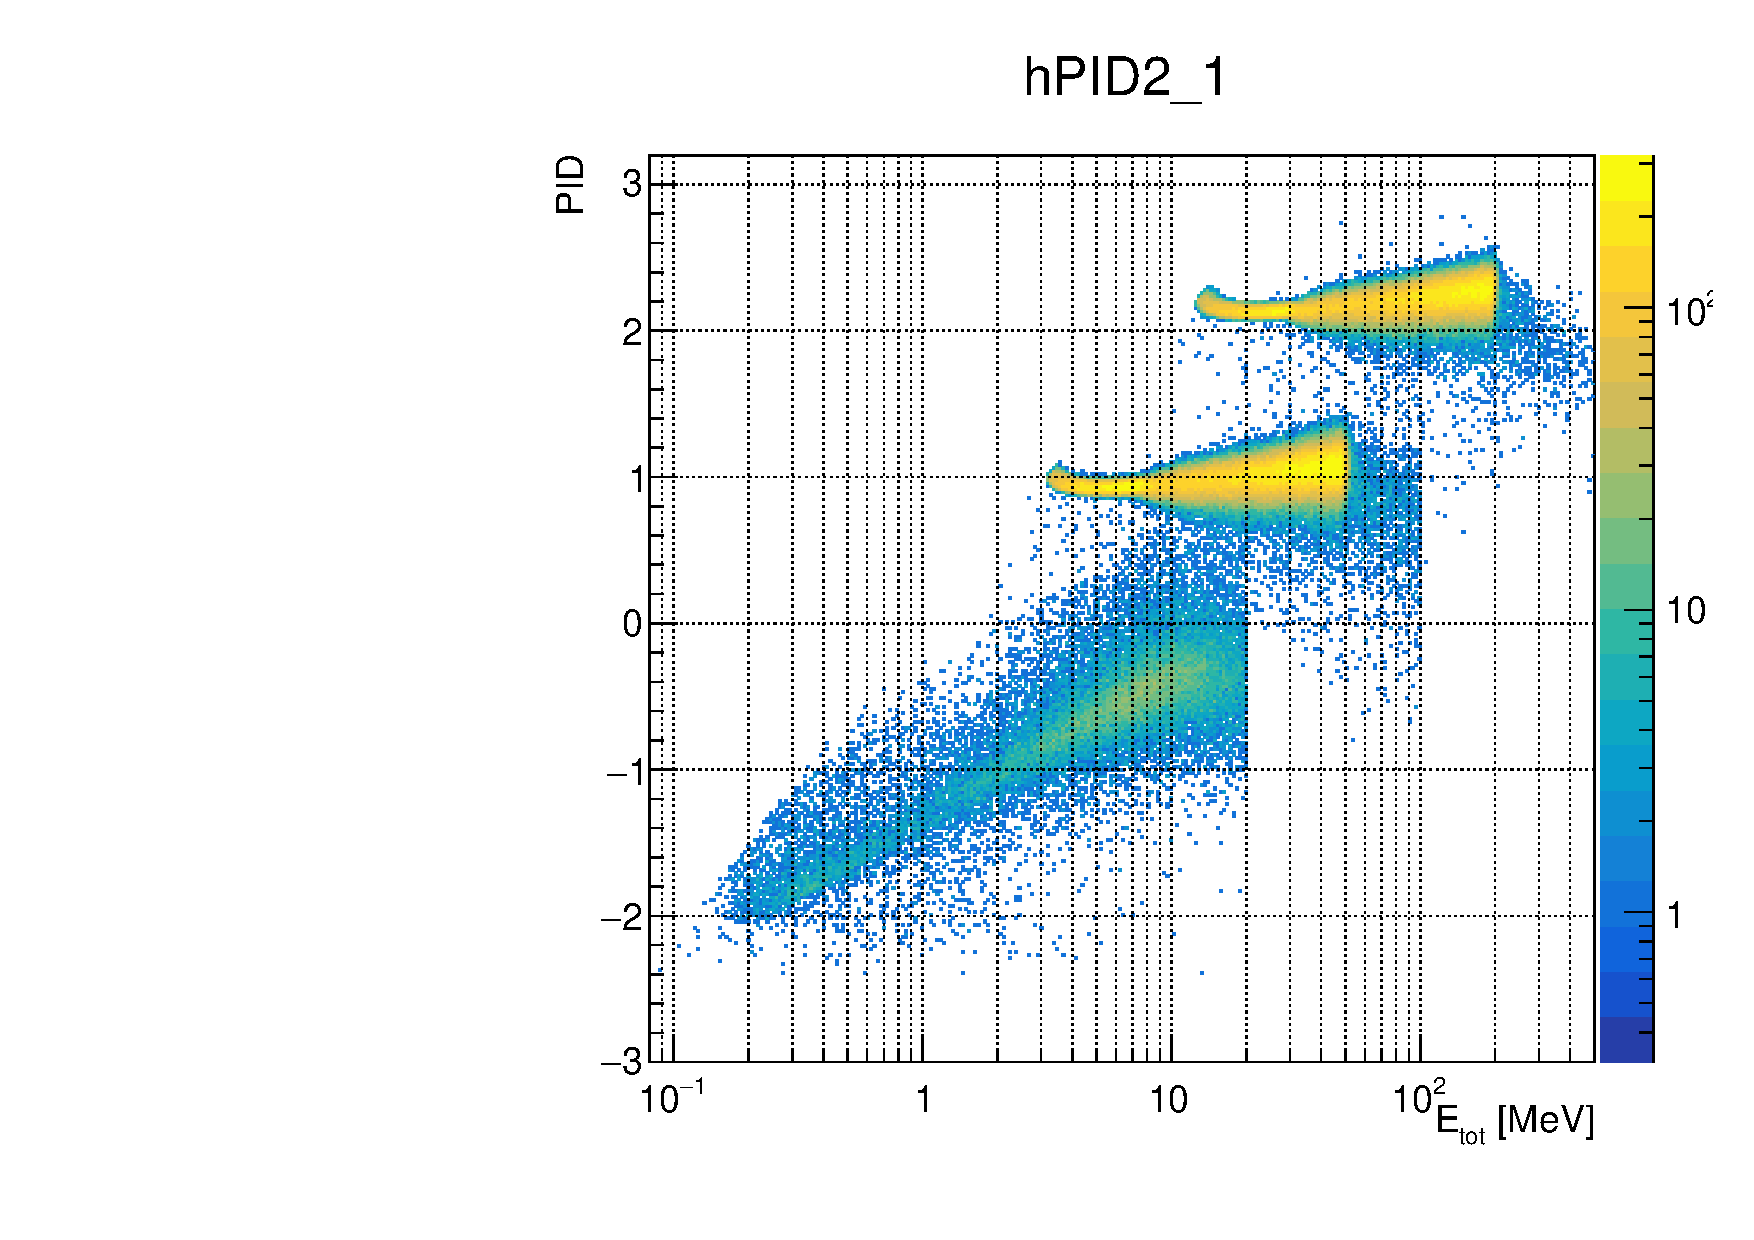
\includegraphics[width=1.0\textwidth]{/home/riccardo/Documenti/GeantProjects/LEM\_GDML\_upgrade/Output\_Geant4Simulation\_20230814/Analysis\_output/GDML\_file\_4/PID\_plots/gPID2.pdf}
            \caption{PID, Gaussian Smearing, Total Energy is the MC Energy.}
        \end{figure}
        
            \end{frame}
            
            \begin{frame}
                \frametitle{PID MC Energy Gaussian Smearing No Calorimeter}
            
        \begin{figure}[h]
            \centering
            \includegraphics[width=1.0\textwidth]{/home/riccardo/Documenti/GeantProjects/LEM\_GDML\_upgrade/Output\_Geant4Simulation\_20230814/Analysis\_output/GDML\_file\_4/PID\_plots/gPID2\_NoCalo.pdf}
            \caption{PID, Gaussian Smearing, Total Energy is the MC Energy, No Calorimeter.}
        \end{figure}
        
            \end{frame}
            
            \begin{frame}
                \frametitle{PID graphs}
            
        \begin{figure}[h]
            \centering
            \includegraphics[width=1.0\textwidth]{/home/riccardo/Documenti/GeantProjects/LEM\_GDML\_upgrade/Output\_Geant4Simulation\_20230814/Analysis\_output/GDML\_file\_4/PID\_plots/graph\_PID\_center.pdf}
            \caption{PID, Gaussian Smearing, Total Energy is the Energy reconstructed, No Calorimeter.}
        \end{figure}
        
            \end{frame}
            
            \begin{frame}
                \frametitle{MC quantities for e-\_t0}
            
        \begin{figure}[h]
            \centering
            \includegraphics[width=1.0\textwidth]{/home/riccardo/Documenti/GeantProjects/LEM\_GDML\_upgrade/Output\_Geant4Simulation\_20230814/Analysis\_output/GDML\_file\_4/Montecarlo\_e-\_t0.pdf}
            \caption{MC quantities}
        \end{figure}
        
            \end{frame}
            
            \begin{frame}
                \frametitle{Energies distribution for e-}
            
        \begin{figure}[h]
            \centering
            \includegraphics[width=1.0\textwidth]{/home/riccardo/Documenti/GeantProjects/LEM\_GDML\_upgrade/Output\_Geant4Simulation\_20230814/Analysis\_output/GDML\_file\_4/Energies\_e-\_t0.pdf}
            \caption{Detected energies}
        \end{figure}
        
            \end{frame}
            
            \begin{frame}
                \frametitle{Angles distribution accepted for e-}
            
        \begin{figure}[h]
            \centering
            \includegraphics[width=1.0\textwidth]{/home/riccardo/Documenti/GeantProjects/LEM\_GDML\_upgrade/Output\_Geant4Simulation\_20230814/Analysis\_output/GDML\_file\_4/Angles\_e-\_t0.pdf}
            \caption{Angles distribution}
        \end{figure}
        
            \end{frame}
            
            \begin{frame}
                \frametitle{Angles distribution accepted for e-}
            
        \begin{figure}[h]
            \centering
            \includegraphics[width=1.0\textwidth]{/home/riccardo/Documenti/GeantProjects/LEM\_GDML\_upgrade/Output\_Geant4Simulation\_20230814/Analysis\_output/GDML\_file\_4/2DAngHistoFigure\_2\_e-\_t0\_e-\_t0.pdf}
            \caption{Angles distribution}
        \end{figure}
        
            \end{frame}
            
            \begin{frame}
                \frametitle{Angles distribution accepted for e-}
            
        \begin{figure}[h]
            \centering
            \includegraphics[width=1.0\textwidth]{/home/riccardo/Documenti/GeantProjects/LEM\_GDML\_upgrade/Output\_Geant4Simulation\_20230814/Analysis\_output/GDML\_file\_4/2DAngHistoFigure\_0\_e-\_t0\_e-\_t0.pdf}
            \caption{Angles distribution}
        \end{figure}
        
            \end{frame}
            
            \begin{frame}
                \frametitle{Angles distribution accepted for e-}
            
        \begin{figure}[h]
            \centering
            \includegraphics[width=1.0\textwidth]{/home/riccardo/Documenti/GeantProjects/LEM\_GDML\_upgrade/Output\_Geant4Simulation\_20230814/Analysis\_output/GDML\_file\_4/2DAngHistoFigure\_3\_e-\_t0\_e-\_t0.pdf}
            \caption{Angles distribution}
        \end{figure}
        
            \end{frame}
            
            \begin{frame}
                \frametitle{Angles distribution accepted for e-}
            
        \begin{figure}[h]
            \centering
            \includegraphics[width=1.0\textwidth]{/home/riccardo/Documenti/GeantProjects/LEM\_GDML\_upgrade/Output\_Geant4Simulation\_20230814/Analysis\_output/GDML\_file\_4/2DAngHistoFigure\_4\_e-\_t0\_e-\_t0.pdf}
            \caption{Angles distribution}
        \end{figure}
        
            \end{frame}
            
            \begin{frame}
                \frametitle{Angles distribution accepted for e-}
            
        \begin{figure}[h]
            \centering
            \includegraphics[width=1.0\textwidth]{/home/riccardo/Documenti/GeantProjects/LEM\_GDML\_upgrade/Output\_Geant4Simulation\_20230814/Analysis\_output/GDML\_file\_4/2DAngHistoFigure\_1\_e-\_t0\_e-\_t0.pdf}
            \caption{Angles distribution}
        \end{figure}
        
            \end{frame}
            
            \begin{frame}
                \frametitle{Generation Position distribution accepted for e-}
            
        \begin{figure}[h]
            \centering
            \includegraphics[width=1.0\textwidth]{/home/riccardo/Documenti/GeantProjects/LEM\_GDML\_upgrade/Output\_Geant4Simulation\_20230814/Analysis\_output/GDML\_file\_4/GenPosition\_2\_e-\_t0\_e-\_t0.pdf}
            \caption{Generation Position}
        \end{figure}
        
            \end{frame}
            
            \begin{frame}
                \frametitle{Generation Position distribution accepted for e-}
            
        \begin{figure}[h]
            \centering
            \includegraphics[width=1.0\textwidth]{/home/riccardo/Documenti/GeantProjects/LEM\_GDML\_upgrade/Output\_Geant4Simulation\_20230814/Analysis\_output/GDML\_file\_4/GenPosition\_0\_e-\_t0\_e-\_t0.pdf}
            \caption{Generation Position}
        \end{figure}
        
            \end{frame}
            
            \begin{frame}
                \frametitle{Generation Position distribution accepted for e-}
            
        \begin{figure}[h]
            \centering
            \includegraphics[width=1.0\textwidth]{/home/riccardo/Documenti/GeantProjects/LEM\_GDML\_upgrade/Output\_Geant4Simulation\_20230814/Analysis\_output/GDML\_file\_4/GenPosition\_3\_e-\_t0\_e-\_t0.pdf}
            \caption{Generation Position}
        \end{figure}
        
            \end{frame}
            
            \begin{frame}
                \frametitle{Generation Position distribution accepted for e-}
            
        \begin{figure}[h]
            \centering
            \includegraphics[width=1.0\textwidth]{/home/riccardo/Documenti/GeantProjects/LEM\_GDML\_upgrade/Output\_Geant4Simulation\_20230814/Analysis\_output/GDML\_file\_4/GenPosition\_1\_e-\_t0\_e-\_t0.pdf}
            \caption{Generation Position}
        \end{figure}
        
            \end{frame}
            
            \begin{frame}
                \frametitle{Generation Position distribution accepted for e-}
            
        \begin{figure}[h]
            \centering
            \includegraphics[width=1.0\textwidth]{/home/riccardo/Documenti/GeantProjects/LEM\_GDML\_upgrade/Output\_Geant4Simulation\_20230814/Analysis\_output/GDML\_file\_4/GenPosition\_4\_e-\_t0\_e-\_t0.pdf}
            \caption{Generation Position}
        \end{figure}
        
            \end{frame}
            
            \begin{frame}
                \frametitle{Geometric factors for e-}
            
            \end{frame}
            
            \begin{frame}
                \frametitle{Geometric factors for e-}
            
            \end{frame}
            
            \begin{frame}
                \frametitle{MC quantities for proton\_t0}
            
        \begin{figure}[h]
            \centering
            \includegraphics[width=1.0\textwidth]{/home/riccardo/Documenti/GeantProjects/LEM\_GDML\_upgrade/Output\_Geant4Simulation\_20230814/Analysis\_output/GDML\_file\_4/Montecarlo\_proton\_t0.pdf}
            \caption{MC quantities}
        \end{figure}
        
            \end{frame}
            
            \begin{frame}
                \frametitle{Energies distribution for proton}
            
        \begin{figure}[h]
            \centering
            \includegraphics[width=1.0\textwidth]{/home/riccardo/Documenti/GeantProjects/LEM\_GDML\_upgrade/Output\_Geant4Simulation\_20230814/Analysis\_output/GDML\_file\_4/Energies\_proton\_t0.pdf}
            \caption{Detected energies}
        \end{figure}
        
            \end{frame}
            
            \begin{frame}
                \frametitle{Angles distribution accepted for proton}
            
        \begin{figure}[h]
            \centering
            \includegraphics[width=1.0\textwidth]{/home/riccardo/Documenti/GeantProjects/LEM\_GDML\_upgrade/Output\_Geant4Simulation\_20230814/Analysis\_output/GDML\_file\_4/Angles\_proton\_t0.pdf}
            \caption{Angles distribution}
        \end{figure}
        
            \end{frame}
            
            \begin{frame}
                \frametitle{Angles distribution accepted for proton}
            
        \begin{figure}[h]
            \centering
            \includegraphics[width=1.0\textwidth]{/home/riccardo/Documenti/GeantProjects/LEM\_GDML\_upgrade/Output\_Geant4Simulation\_20230814/Analysis\_output/GDML\_file\_4/2DAngHistoFigure\_0\_proton\_t0\_proton\_t0.pdf}
            \caption{Angles distribution}
        \end{figure}
        
            \end{frame}
            
            \begin{frame}
                \frametitle{Angles distribution accepted for proton}
            
        \begin{figure}[h]
            \centering
            \includegraphics[width=1.0\textwidth]{/home/riccardo/Documenti/GeantProjects/LEM\_GDML\_upgrade/Output\_Geant4Simulation\_20230814/Analysis\_output/GDML\_file\_4/2DAngHistoFigure\_4\_proton\_t0\_proton\_t0.pdf}
            \caption{Angles distribution}
        \end{figure}
        
            \end{frame}
            
            \begin{frame}
                \frametitle{Angles distribution accepted for proton}
            
        \begin{figure}[h]
            \centering
            \includegraphics[width=1.0\textwidth]{/home/riccardo/Documenti/GeantProjects/LEM\_GDML\_upgrade/Output\_Geant4Simulation\_20230814/Analysis\_output/GDML\_file\_4/2DAngHistoFigure\_3\_proton\_t0\_proton\_t0.pdf}
            \caption{Angles distribution}
        \end{figure}
        
            \end{frame}
            
            \begin{frame}
                \frametitle{Angles distribution accepted for proton}
            
        \begin{figure}[h]
            \centering
            \includegraphics[width=1.0\textwidth]{/home/riccardo/Documenti/GeantProjects/LEM\_GDML\_upgrade/Output\_Geant4Simulation\_20230814/Analysis\_output/GDML\_file\_4/2DAngHistoFigure\_2\_proton\_t0\_proton\_t0.pdf}
            \caption{Angles distribution}
        \end{figure}
        
            \end{frame}
            
            \begin{frame}
                \frametitle{Angles distribution accepted for proton}
            
        \begin{figure}[h]
            \centering
            \includegraphics[width=1.0\textwidth]{/home/riccardo/Documenti/GeantProjects/LEM\_GDML\_upgrade/Output\_Geant4Simulation\_20230814/Analysis\_output/GDML\_file\_4/2DAngHistoFigure\_1\_proton\_t0\_proton\_t0.pdf}
            \caption{Angles distribution}
        \end{figure}
        
            \end{frame}
            
            \begin{frame}
                \frametitle{Generation Position distribution accepted for proton}
            
        \begin{figure}[h]
            \centering
            \includegraphics[width=1.0\textwidth]{/home/riccardo/Documenti/GeantProjects/LEM\_GDML\_upgrade/Output\_Geant4Simulation\_20230814/Analysis\_output/GDML\_file\_4/GenPosition\_1\_proton\_t0\_proton\_t0.pdf}
            \caption{Generation Position}
        \end{figure}
        
            \end{frame}
            
            \begin{frame}
                \frametitle{Generation Position distribution accepted for proton}
            
        \begin{figure}[h]
            \centering
            \includegraphics[width=1.0\textwidth]{/home/riccardo/Documenti/GeantProjects/LEM\_GDML\_upgrade/Output\_Geant4Simulation\_20230814/Analysis\_output/GDML\_file\_4/GenPosition\_2\_proton\_t0\_proton\_t0.pdf}
            \caption{Generation Position}
        \end{figure}
        
            \end{frame}
            
            \begin{frame}
                \frametitle{Generation Position distribution accepted for proton}
            
        \begin{figure}[h]
            \centering
            \includegraphics[width=1.0\textwidth]{/home/riccardo/Documenti/GeantProjects/LEM\_GDML\_upgrade/Output\_Geant4Simulation\_20230814/Analysis\_output/GDML\_file\_4/GenPosition\_4\_proton\_t0\_proton\_t0.pdf}
            \caption{Generation Position}
        \end{figure}
        
            \end{frame}
            
            \begin{frame}
                \frametitle{Generation Position distribution accepted for proton}
            
        \begin{figure}[h]
            \centering
            \includegraphics[width=1.0\textwidth]{/home/riccardo/Documenti/GeantProjects/LEM\_GDML\_upgrade/Output\_Geant4Simulation\_20230814/Analysis\_output/GDML\_file\_4/GenPosition\_3\_proton\_t0\_proton\_t0.pdf}
            \caption{Generation Position}
        \end{figure}
        
            \end{frame}
            
            \begin{frame}
                \frametitle{Generation Position distribution accepted for proton}
            
        \begin{figure}[h]
            \centering
            \includegraphics[width=1.0\textwidth]{/home/riccardo/Documenti/GeantProjects/LEM\_GDML\_upgrade/Output\_Geant4Simulation\_20230814/Analysis\_output/GDML\_file\_4/GenPosition\_0\_proton\_t0\_proton\_t0.pdf}
            \caption{Generation Position}
        \end{figure}
        
            \end{frame}
            
            \begin{frame}
                \frametitle{Geometric factors for proton}
            
            \end{frame}
            
            \begin{frame}
                \frametitle{Geometric factors for proton}
            
            \end{frame}
            
            \begin{frame}
                \frametitle{MC quantities for alpha\_t0}
            
        \begin{figure}[h]
            \centering
            \includegraphics[width=1.0\textwidth]{/home/riccardo/Documenti/GeantProjects/LEM\_GDML\_upgrade/Output\_Geant4Simulation\_20230814/Analysis\_output/GDML\_file\_4/Montecarlo\_alpha\_t0.pdf}
            \caption{MC quantities}
        \end{figure}
        
            \end{frame}
            
            \begin{frame}
                \frametitle{Energies distribution for alpha}
            
        \begin{figure}[h]
            \centering
            \includegraphics[width=1.0\textwidth]{/home/riccardo/Documenti/GeantProjects/LEM\_GDML\_upgrade/Output\_Geant4Simulation\_20230814/Analysis\_output/GDML\_file\_4/Energies\_alpha\_t0.pdf}
            \caption{Detected energies}
        \end{figure}
        
            \end{frame}
            
            \begin{frame}
                \frametitle{Angles distribution accepted for alpha}
            
        \begin{figure}[h]
            \centering
            \includegraphics[width=1.0\textwidth]{/home/riccardo/Documenti/GeantProjects/LEM\_GDML\_upgrade/Output\_Geant4Simulation\_20230814/Analysis\_output/GDML\_file\_4/Angles\_alpha\_t0.pdf}
            \caption{Angles distribution}
        \end{figure}
        
            \end{frame}
            
            \begin{frame}
                \frametitle{Angles distribution accepted for alpha}
            
        \begin{figure}[h]
            \centering
            \includegraphics[width=1.0\textwidth]{/home/riccardo/Documenti/GeantProjects/LEM\_GDML\_upgrade/Output\_Geant4Simulation\_20230814/Analysis\_output/GDML\_file\_4/2DAngHistoFigure\_3\_alpha\_t0\_alpha\_t0.pdf}
            \caption{Angles distribution}
        \end{figure}
        
            \end{frame}
            
            \begin{frame}
                \frametitle{Angles distribution accepted for alpha}
            
        \begin{figure}[h]
            \centering
            \includegraphics[width=1.0\textwidth]{/home/riccardo/Documenti/GeantProjects/LEM\_GDML\_upgrade/Output\_Geant4Simulation\_20230814/Analysis\_output/GDML\_file\_4/2DAngHistoFigure\_4\_alpha\_t0\_alpha\_t0.pdf}
            \caption{Angles distribution}
        \end{figure}
        
            \end{frame}
            
            \begin{frame}
                \frametitle{Angles distribution accepted for alpha}
            
        \begin{figure}[h]
            \centering
            \includegraphics[width=1.0\textwidth]{/home/riccardo/Documenti/GeantProjects/LEM\_GDML\_upgrade/Output\_Geant4Simulation\_20230814/Analysis\_output/GDML\_file\_4/2DAngHistoFigure\_2\_alpha\_t0\_alpha\_t0.pdf}
            \caption{Angles distribution}
        \end{figure}
        
            \end{frame}
            
            \begin{frame}
                \frametitle{Angles distribution accepted for alpha}
            
        \begin{figure}[h]
            \centering
            \includegraphics[width=1.0\textwidth]{/home/riccardo/Documenti/GeantProjects/LEM\_GDML\_upgrade/Output\_Geant4Simulation\_20230814/Analysis\_output/GDML\_file\_4/2DAngHistoFigure\_1\_alpha\_t0\_alpha\_t0.pdf}
            \caption{Angles distribution}
        \end{figure}
        
            \end{frame}
            
            \begin{frame}
                \frametitle{Angles distribution accepted for alpha}
            
        \begin{figure}[h]
            \centering
            \includegraphics[width=1.0\textwidth]{/home/riccardo/Documenti/GeantProjects/LEM\_GDML\_upgrade/Output\_Geant4Simulation\_20230814/Analysis\_output/GDML\_file\_4/2DAngHistoFigure\_0\_alpha\_t0\_alpha\_t0.pdf}
            \caption{Angles distribution}
        \end{figure}
        
            \end{frame}
            
            \begin{frame}
                \frametitle{Generation Position distribution accepted for alpha}
            
        \begin{figure}[h]
            \centering
            \includegraphics[width=1.0\textwidth]{/home/riccardo/Documenti/GeantProjects/LEM\_GDML\_upgrade/Output\_Geant4Simulation\_20230814/Analysis\_output/GDML\_file\_4/GenPosition\_1\_alpha\_t0\_alpha\_t0.pdf}
            \caption{Generation Position}
        \end{figure}
        
            \end{frame}
            
            \begin{frame}
                \frametitle{Generation Position distribution accepted for alpha}
            
        \begin{figure}[h]
            \centering
            \includegraphics[width=1.0\textwidth]{/home/riccardo/Documenti/GeantProjects/LEM\_GDML\_upgrade/Output\_Geant4Simulation\_20230814/Analysis\_output/GDML\_file\_4/GenPosition\_2\_alpha\_t0\_alpha\_t0.pdf}
            \caption{Generation Position}
        \end{figure}
        
            \end{frame}
            
            \begin{frame}
                \frametitle{Generation Position distribution accepted for alpha}
            
        \begin{figure}[h]
            \centering
            \includegraphics[width=1.0\textwidth]{/home/riccardo/Documenti/GeantProjects/LEM\_GDML\_upgrade/Output\_Geant4Simulation\_20230814/Analysis\_output/GDML\_file\_4/GenPosition\_3\_alpha\_t0\_alpha\_t0.pdf}
            \caption{Generation Position}
        \end{figure}
        
            \end{frame}
            
            \begin{frame}
                \frametitle{Generation Position distribution accepted for alpha}
            
        \begin{figure}[h]
            \centering
            \includegraphics[width=1.0\textwidth]{/home/riccardo/Documenti/GeantProjects/LEM\_GDML\_upgrade/Output\_Geant4Simulation\_20230814/Analysis\_output/GDML\_file\_4/GenPosition\_0\_alpha\_t0\_alpha\_t0.pdf}
            \caption{Generation Position}
        \end{figure}
        
            \end{frame}
            
            \begin{frame}
                \frametitle{Generation Position distribution accepted for alpha}
            
        \begin{figure}[h]
            \centering
            \includegraphics[width=1.0\textwidth]{/home/riccardo/Documenti/GeantProjects/LEM\_GDML\_upgrade/Output\_Geant4Simulation\_20230814/Analysis\_output/GDML\_file\_4/GenPosition\_4\_alpha\_t0\_alpha\_t0.pdf}
            \caption{Generation Position}
        \end{figure}
        
            \end{frame}
            
            \begin{frame}
                \frametitle{Geometric factors for alpha}
            
            \end{frame}
            
            \begin{frame}
                \frametitle{Geometric factors for alpha}
            
            \end{frame}
            
            \begin{frame}
                \frametitle{Geometric factors for all particles}
            
            \end{frame}
            
        \end{document}
        